\documentclass[12pt]{article}
\usepackage[left=3cm, right=3cm, top=3cm]{geometry}
\usepackage{amsmath}
\usepackage{graphicx}
\usepackage{hyperref}
\usepackage{subcaption}
\usepackage{wrapfig}
\usepackage[latin1]{inputenc}

\setlength{\parindent}{0cm}

\title{ECEN303 Force Balance Scale}
\author{Celine Jane  300400152, Mohammad Al-rubayee}


\begin{document}
	\maketitle
	\section{Abstract}
	- results of entire project 
	\section{Introduction}
	- describe project \\
	- specifications
	\section{Background}
	- description of speaker and optical sensors\\
	- how force balance works \\
	- op amps ???? idk
	
	\newpage
	
	\section{Method}
	
	\begin{wrapfigure}{r}{0.5\columnwidth}
		\centering
		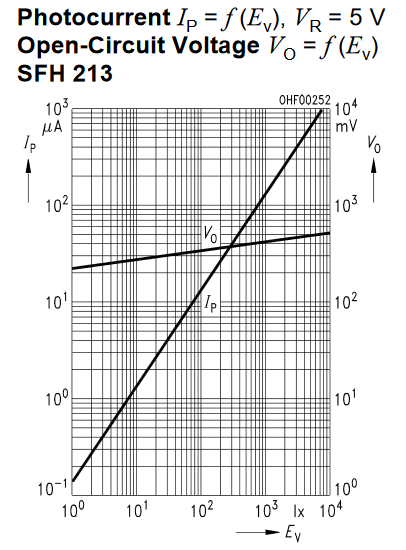
\includegraphics{photocurrent}
		\caption{Photocurrent Information from Datasheet[1]}
		
	\end{wrapfigure}
	
	The scale has 5 main blocks - a transimpedance amplifier, a low pass filter, an instrumentation amplifier, a summing amplifier and a sample and hold circuit.
	
	\subsection{Transimpedance Amplifier and Low-Pass Filter}
	
	The output current of the two optical sensors changes as the speaker moves up and down. As seen in Figure 1, the output is in the micro-amp range. The transimpedance amplifier outputs a voltage that is controlled by the input current, as well as amplifying the input to a more usable milli-volt range. The output voltage can be described by the equation
	$$ V_{O} = -Ri_{I}$$
	Where R is a feedback resistor and $i_{I}$ is the input source current. To get outputs in the milli-volt range, a resistance of $560k\Omega$ is chosen as the feedback resistance. \\
	
	The op-amp chosen for the transimpedance amplifier is the LM348N. This was chosen for its low input voltage and current offsets. If the input current offset was high, this would have a large effect on the input source current because the magnitude is so small. \\
	
	To filter out unwanted frequencies on the output (the output should ideally be a DC signal), a passive low-pass filter is attached to the output of the transimpedance amplifier. Using a resistance of $150k\Omega$ and a capacitance of $0.1\mu F$, the cutoff frequency can be found:
	$$f_{c} = \frac{1}{2\pi\cdot RC}$$ \\
	$$ = \frac{1}{2\pi\cdot 150k\Omega\cdot0.1\mu F} $$ \\
	$$ = 10.6 Hz$$ \\
	The resulting transimpedance amplifier and low pass filter design can be seen in Figure 2, where $I_{1}$ is the input from one of the optical emitters. The second optical emitter current is not shown, but the circuit is the same.
	\begin{figure}[h]
		\centering
		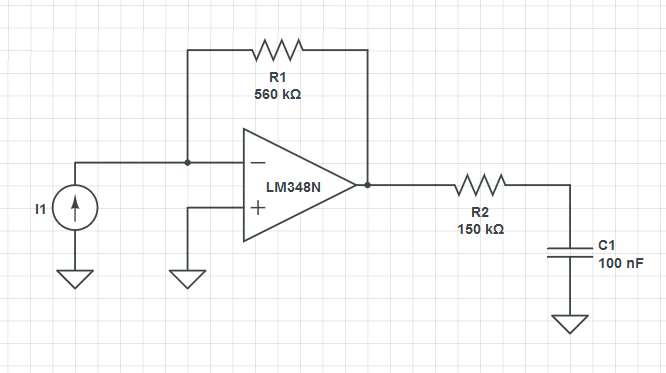
\includegraphics[width=\columnwidth]{transimpedance_lpf}
		\caption{Transimpedance Amplifer and Low Pass Filter}
	\end{figure}
	
	\subsection{Instrumentation Amplifier and Summing Amplifier}
	The instrumentation amplifier outputs a measure of how the two optical emitter currents differ. Ideally, when the speaker position is at it 0 level (no weight), the difference between the emitters would be 0. As more weight is added onto the speaker, the difference would increase. However in reality the speaker has an offset at its 0 position so the difference between the emitters actually decreases as more weight is added. This is why there is a summing amplifier after the instrumentation amplifier. \\
	
	The gain of the instrumentation amplifier is controlled by the resistor $R_{G}$. For this circuit, $R_{G}$ is a trim pot so that the gain can be adjusted during testing. \\
	
	Instrumentation amplifiers can be bought on a single chip however due to costs, the amplifier was built using external resistors and a LM348N chip.\\
	
	The output of a summing amplifier is
	$$V_{O} = \frac{-R_{f}}{R_{in}}(V_{A}+V_{in})$$
	Where $V_{A}$ is the output of the instrumentation amplifier and $V_{in}$ is an adjustable voltage from a power supply. If $V_{in}$ is a negative voltage, then the output will increase as more weight is added. $V_{in}$ should be adjusted so that at the speaker 0 level, the output voltage is 0V. The resulting circuit can be seen in Figure 3.\\
	
	FIGURE 3 !!!
	
	\subsection{Sample and Hold}
	The functionality of the sample and hold circuit is to output a voltage that will change the level of the speaker until it reaches its 0 position. At this point it will hold the zeroing voltage constant until the level of the speaker is changed again. 
	
	The sample and hold circuit can be seen in Figure 4\\
	
	Figure 4 !!!!!\\
	
	\begin{wrapfigure}{l}{0.5\columnwidth}
		\centering
		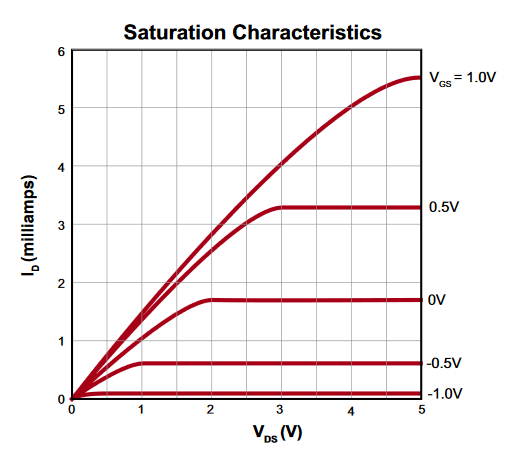
\includegraphics[width=0.5\columnwidth]{mosfet}
		\caption{Saturation Characteristics from Datasheet[3]}
	\end{wrapfigure}
	
	The output of the summing amplifier is the input into the comparator and first voltage follower. The comparator will output a constant voltage to the gate of the N-MOSFET, where it will conduct based on the source voltage (the output of the voltage follower). If the output of the summing amplifier is 0 (e.g the speaker has reached its zero position), then the output of the comparator will be 0, turning the MOSFET off so that it will no longer conduct.\\
	
	When the comparator turns off, the capacitor will hold the output voltage and the speaker will be held at its 0 position.\\
	
	The transistor used is the LND150N3-G. This was chosen specifically for its drain current being in the milli-amps range. As seen in Figure 5, $V_{GS}$ will be at 1V, supplied by the comparator. $V_{DS}$ will be the output from the summing amplifier and will be in the linear region so that larger differences (i.e more weight is on the speaker) will produce larger balancing forces. \\
	
	The comparator used is the LM2901. This was chosen because the output can go as low as 1V and has 0V as its reference voltage, so that when the speaker is at its 0 position, the difference is 0V and the comparator will turn off the MOSFET. 
	
	The voltage follower on the output also ensures that enough supply current can be supplied to the speaker. 
	
	\subsection{Overweight Indicator}
	If an object placed on the speaker is overweight, then an LED will turn on. The resistance used is a trim pot, so that the set point for being overweight is adjustable. \\
	
	FIGURE ?? - TRIM POT AND LED
	
	\subsection{PCB Design and Layout}
	As seen in Figure ??, the PCB is laid out based on the functional blocks. Some functional blocks are combined because they share the same op-amp chip.\\ 
	
	Bypass capacitors are used on the supply rails and supply rail pin inputs. A large capacitance of $1\mu F$ is used on the supply rails to ensure a smooth supply voltage. The bypass capacitors on the input pins are at $100pF$ to supply current spikes to the chip if needed.\\
	
	FIGURE ??? PCB
	
	\subsection{Speaker Characteristics}
	In order to adjust the force-balance circuit to accurately counter the weight, some characteristics need to measured. The output of the emitters and different weights were measured, to determine the difference between the two. Using this knowledge, the voltage and current required to move the speaker back to the zero level at different weights was measured. 
	
	\section{Results}
		\subsection{Transimpedance Amplifier and Low Pass Filter}
		The output from the transimpedance amplifiers, connected to the optical emitters, can be seen in Figure ????.
		
		\begin{figure}[h]
			\centering
			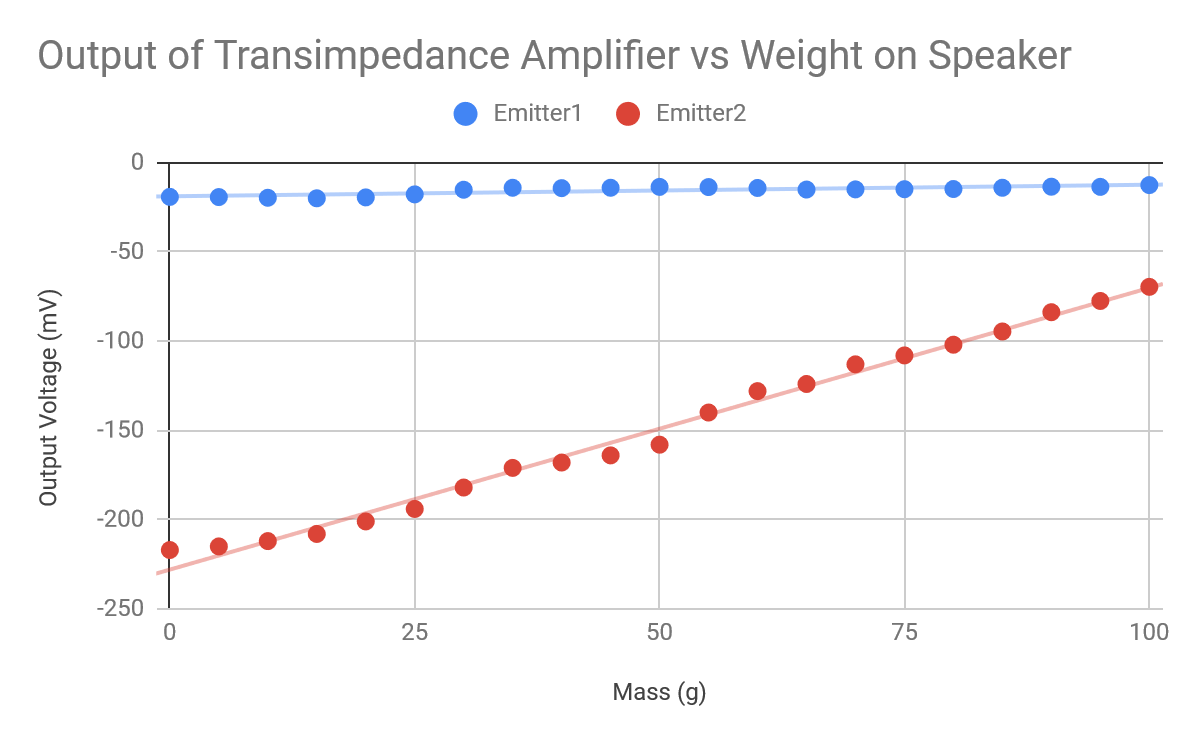
\includegraphics[width=\columnwidth]{transimpedance_results}
			\caption{}
		\end{figure}
		
		Both outputs are negative, as dictated by the nature of this amplifier. The voltage from emitter 1 does not change as more weight is added whereas the output from emitter 2 increases with weight.\\
		
		As seen in Figure ???, the low pass filter reduces the amount of oscillations.\\
		
		FIGURE ??? - LPF RESULTS, before and after photo 
		
		\subsection{Instrumentation and Summing Amplifier}
		The difference between the emitters can be seen in Figure ???. This specific Figure is with a unity gain, but is adjustable for the testing process. Regardless of the gain, the relationship between the mass and voltage difference is inversely proportional.\\
		\begin{figure}[h!]
			\centering
			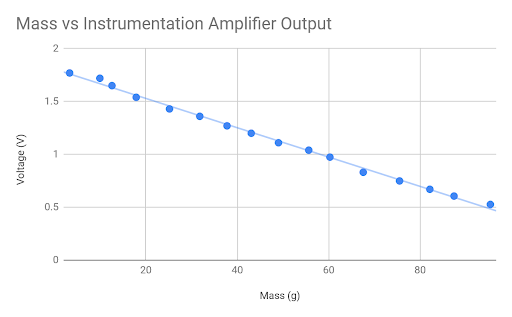
\includegraphics[width=\columnwidth]{difference_results}
			\caption{}
		\end{figure}
		
		SUMMING AMPLIFIER RESULTS: does it make the relationship proportional???
		\subsection{Sample and Hold}
		
		RESULTS: comparator output vs input from summing amp, output of sample and hold vs summing amp input
		
		\subsection{Overweight Indicator}
		did it light up at 100g?
		
		\subsection{Speaker Characteristics}
		Figure ??? shows the required voltage and current levels needed to hold the speaker at its 0 position when different weights are added. Both voltage and current are proportional with time. The voltage required is approximately 10mV per gram added.
		\begin{figure}[h!]
			\centering
			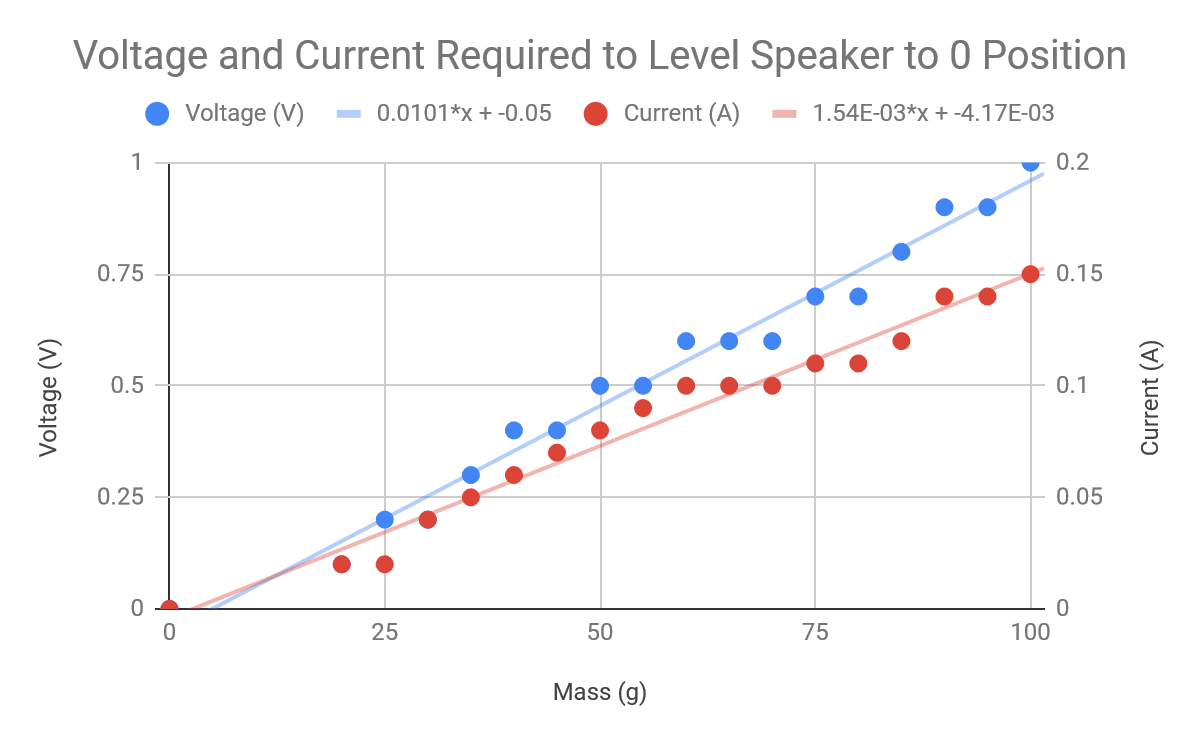
\includegraphics[width=\columnwidth]{speaker}
			\caption{}
		\end{figure}
		
		
	\section{Discussion}
	- does it work tho, if not - why ?\\
	- did it meet all the specifications?
	\section{Conclusion}
	- has some functionality, needs more work\\
	- doesn't meet all the specifications.
	
	\section{References}
	\section{Contributions}
	
	\section{Appendices}
	schematic, PCB, BOM
\end{document}